\documentclass[margin=0.5mm]{standalone}
\usepackage{pgfplots}
\usetikzlibrary{pgfplots.groupplots}
\pgfplotsset{compat=1.7}

\begin{document}
	\thispagestyle{empty}
	
%	\begin{figure}[t]
%		\centering
		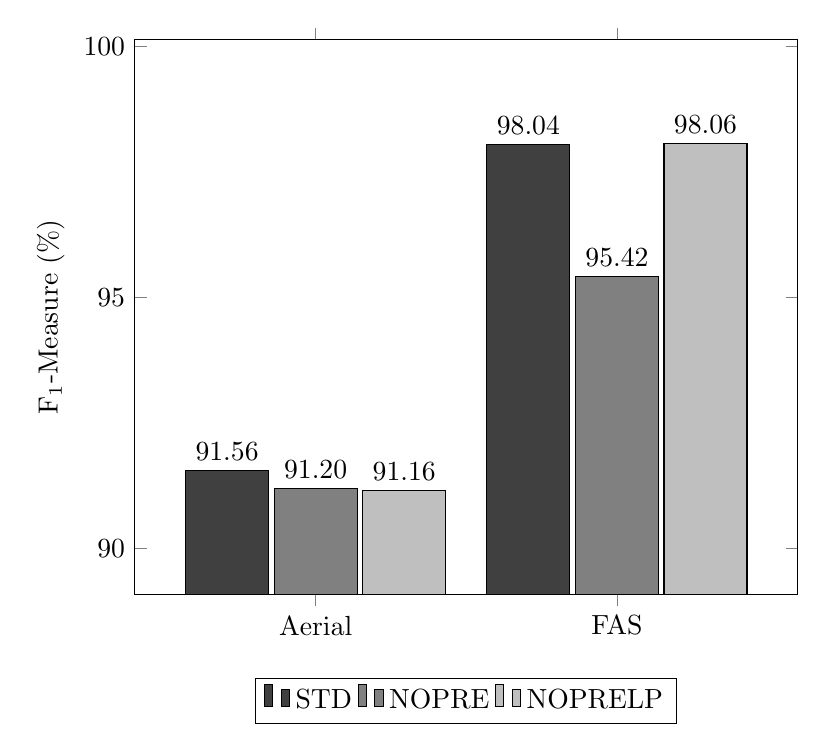
\begin{tikzpicture}
		\begin{axis}[
		width=10cm,
		enlarge x limits=0.6,
		enlarge y limits=0.3,
			ybar,
			legend style={at={(0.5,-0.15)},
				anchor=north,legend columns=-1},
			ylabel={F$_1$-Measure (\%)},
			symbolic x coords={Aerial,FAS},
			xtick=data,
		  nodes near coords={\pgfmathprintnumber[fixed zerofill, precision=2]{\pgfplotspointmeta}},
			nodes near coords align={vertical},
			bar width=30pt,
			style={font=\normalsize},
			ytick={80,85,...,100}
		]
		%						STD		NPRE	NOPRELP
		%			Aerial
		%				Clean	91.56	91.20	91.16
		%				Noisy   84.57   84.49	78.22
		
		%			FAS		
		%				Clean	98.04	95.42	98.06
		%				Noisy   85.94	89.93	89.24
		
		
		\addplot [color=black,fill=darkgray] coordinates {(Aerial,91.56) (FAS,98.04)  };
		\addplot [color=black,fill=gray] coordinates {(Aerial,91.20) (FAS,95.42) };
		\addplot [color=black,fill=lightgray] coordinates {(Aerial,91.16) (FAS,98.06) };		
		
		\legend{STD,NOPRE,NOPRELP}
		\end{axis}
		\end{tikzpicture}
		
		%\vspace{-0.7cm}
		%\caption{Left: the pitch distribution for the 10 male speakers. Right: the active speech level for the 20 speakers.}\label{fig:pitch}
		%\vspace{-0.5cm}
%	\end{figure}
\end{document}